\section{\textsc{Rührei}}

\subsection*{Zutaten für 2 Portionen:}

\begin{tabular}{p{7.5cm} p{7.5cm}}
	& \\
	6 Eier & 250ml Milch \\
	2EL Öl & Salz, Pfeffer, Muskatnuss
\end{tabular}

\subsection*{Serviervorschlag:}

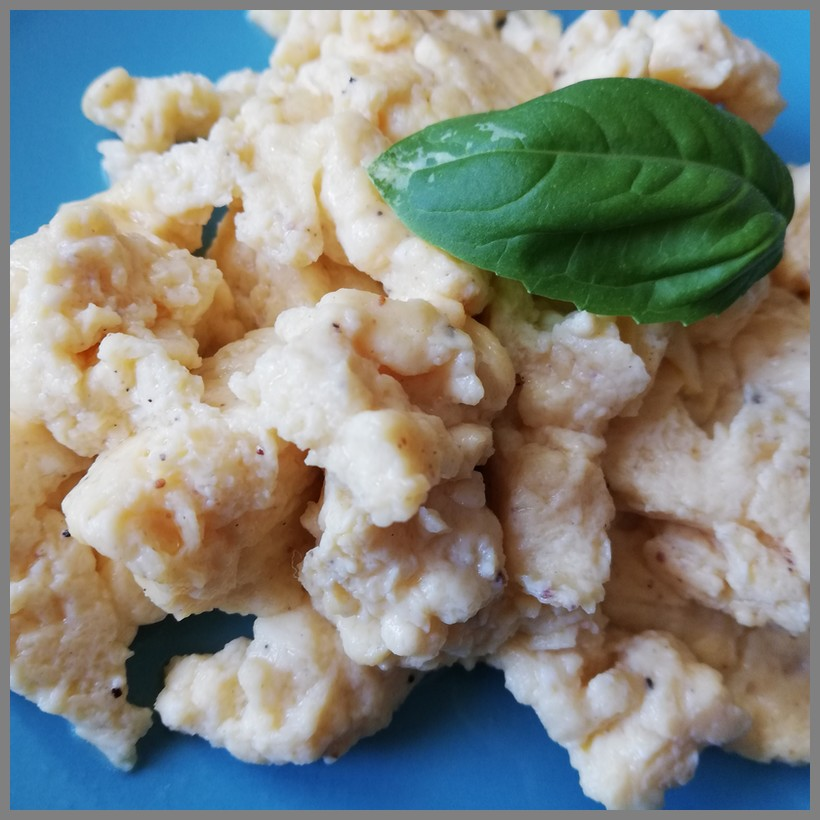
\includegraphics[width=\textwidth]{img/ruehrei.jpg} \cite{ruehrei}

\subsection*{So geht's:}

\begin{tabular}{p{15cm}}
	\\
	Die Milch in einem Messbecher abfüllen. Die Eier auch in diesen schlagen. Mit einem Schneebesen zu einer glatten Masse rühren.\\
	Je nach Geschmack mit Salz, Pfeffer und Muskatnuss würzen.\\
	Öl in einer Pfanne erhitzen. Die gesamte Eimasse hineingeben.\\
	Kurz stocken lassen. Das Ei nun mit einem Pfannenschaber von innen nach außen schieben. Vorgang so lange wiederholen, bis das gesamte Ei gestockt ist.
\end{tabular}
